\documentclass[onecolumn, letter, 11pt]{article}

\usepackage{fourier}
\usepackage[utf8]{inputenc}
\usepackage[sumlimits]{amsmath}
\usepackage{graphicx}
\usepackage[spanish]{babel}
\usepackage{amsfonts}
\usepackage{amssymb}
\usepackage{amsthm}
\usepackage{geometry}

\geometry{left=2.5cm,right=2.5cm,top=2.5cm,bottom=2.5cm}


\title{Examen rápido No. 7}
\author{Inteligencia Artificial\\ \textsc{Julio Waissman Vilanova}}
\date{}


\begin{document}

\maketitle

\section*{Un árbol de juego muy básico}

Considere el siguiente juego:

\begin{center}
\begin{tabular}{|c|c|c|c|c|}
\hline
A& & & &B\\
\hline
\end{tabular}
\end{center}
donde el jugador A siempre comienza el juego. Un jugador puede moverse
en cada juego a una casilla adjacente a la que se encuentra, o, si en
la casilla adjacente se encuentra el jugador contrario, lo brinca a la
siguiente casilla.

Responde las siguientes preguntas (10 puntos por inciso):
\begin{itemize}
\item Dibuja el árbol de juego para este juego hasta una profundidad 7. ¿El árbol es finito?
  ¿Porqué?
\item ¿Como modificarías el algoritmo Minimax para que este tipo de
  juegos tuviera una búsqueda pequeña? ¿Cual sería la ventaja? ¿Que
  desventajas tendría?
\item De acuerdo a tu nueva representación, ¿Algún jugador ganaría
  siempre el juego? ¿Quien?
\end{itemize}

\newpage

\section*{Podando con $\alpha$--$\beta$}
Marca en el siguiente árbol de juego las ramas que serían podadas en una búsqueda minimax
con poda $\alpha$--$\beta$ si la exploración se realiza siempre primero el nodo más a la
izquierda (los nodos $\triangle$ son nodos del jugador \emph{max} y los nodos
$\triangledown$ son los que corresponden a un jugador \emph{min}) (35 puntos).

\begin{center}
  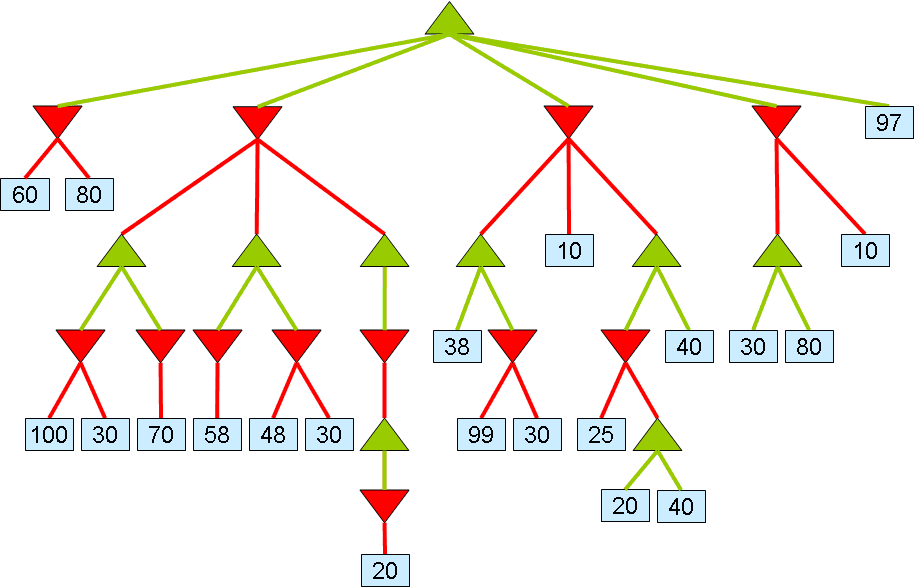
\includegraphics[width = 0.8\textwidth]{minimax_tree_1.png}
\end{center}

Si el orden en que se seleccionan las jugadas del nodo raíz se modifica levemente, marca las ramas
que serían podadas en el árbol, arreglado de la siguiente forma (35 puntos):

\begin{center}
  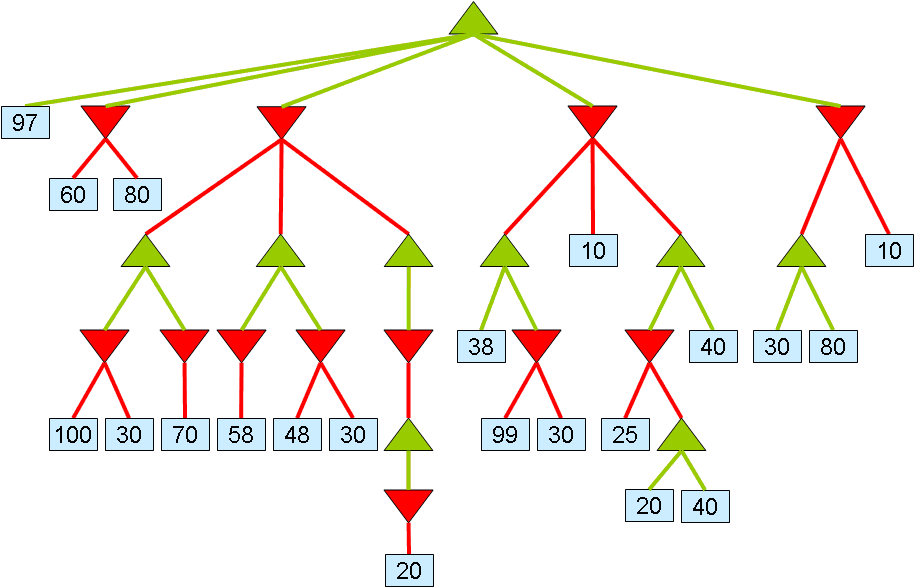
\includegraphics[width = 0.8\textwidth]{minimax_tree_2.png}
\end{center}


\end{document}
